% Author: Izaak Neutelings (July 2018)
\documentclass[border=3pt,tikz]{standalone}
\usepackage{tikz}
\usepackage{physics}
\usepackage{esvect}
\tikzset{>=latex} % for LaTeX arrow head
\usetikzlibrary{angles,quotes} % for pic (angle labels)
\usepackage{xcolor}
\colorlet{pinkskin}{pink!25}
\colorlet{brownskin}{pink!5!brown!45}
\colorlet{myred}{red!90!black}
\colorlet{myblue}{blue!90!black}
\colorlet{mypurple}{blue!50!red!80!black!80}
\colorlet{Bcol}{violet!90}
\colorlet{BFcol}{red!60!black}
\colorlet{veccol}{green!45!black}
\colorlet{Icol}{blue!70!black}
\colorlet{mucol}{red!90!black}
\tikzstyle{BField}=[->,line width=2,Bcol]
\tikzstyle{current}=[->,line width=2,Icol] %thick,
\tikzstyle{force}=[->,line width=2,BFcol]
\tikzstyle{vector}=[->,line width=2,veccol]
\tikzstyle{thick vector}=[->,line width=2,veccol]
\tikzstyle{mu vector}=[->,line width=2,mucol]
\tikzstyle{velocity}=[->,line width=2,veccol]
\tikzstyle{charge+}=[very thin,draw=black,top color=red!50,bottom color=red!90!black,shading angle=20,circle,inner sep=0.5]


\begin{document}

% RIGHT HAND RULE - magnetic moment
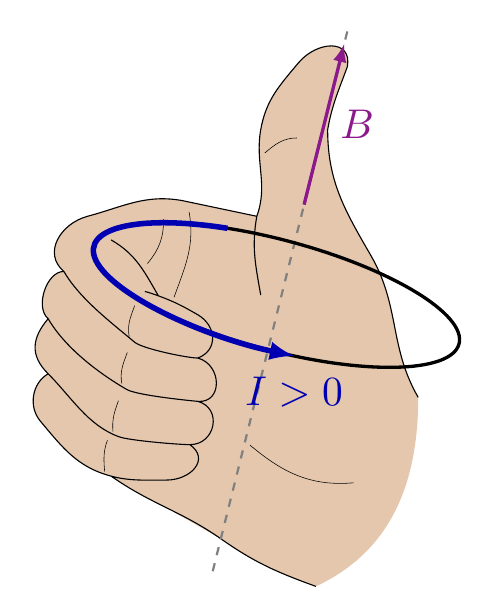
\begin{tikzpicture}
  \coordinate (O) at (1.1,0.2); % ORIGIN
  \coordinate (WT) at ( 2.9,-1.1); % WRIST TOP
  \coordinate (T1) at ( 2.3, 0.7); % THUMB
  \coordinate (T2) at ( 1.75, 2.3);
  \coordinate (T3) at ( 2.0, 3.1);
  \coordinate (T4) at (1.38, 3.15);
  \coordinate (T5) at ( 0.9, 2.3);
  \coordinate (T6) at ( 0.85, 1.2);
  \coordinate (T7) at ( 0.9, 0.2);
  \coordinate (I1) at (-0.1, 1.4); % INDEX
  \coordinate (I2) at (-1.3, 1.2);
  \coordinate (I3) at (-1.6, 0.5);
  \coordinate (I4) at (-0.7,-0.4);
  \coordinate (I5) at ( 0.1,-0.6);
  \coordinate (I6) at ( 0.1,-0.05);
  \coordinate (I7) at (-0.4,0.19);
  \coordinate (I8) at (-1.0, 0.9);
  \coordinate (M1) at (-1.8,-0.1); % MIDDLE
  %\coordinate (M2) at (-0.5,-0.7);
  \coordinate (M2) at (-0.8,-1.0);
  \coordinate (M3) at ( 0.1,-1.15);
  \coordinate (R1) at (-1.8,-0.8); % RING
  \coordinate (R2) at (-0.9,-1.6);
  \coordinate (R3) at (-0.0,-1.7);
  \coordinate (R4) at ( 0.0,-1.1);
  \coordinate (P1) at (-1.9,-1.4); % PINKY
  \coordinate (P2) at (-1.0,-2.1);
  \coordinate (P3) at (-0.3,-2.15);
  \coordinate (W1) at ( 0.4,-2.9); % WRIST BOTTOM
  \coordinate (W2) at ( 1.6,-3.5);
  
  % HAND
  \fill[brownskin]
    (WT) -- (T6) -- (I2) -- (P2) -- (W1) -- (W2) to[out=25,in=-90] cycle;
  \draw[fill=brownskin]
    (WT) to[out=120,in=-60] % THUMB
    (T1) to[out=120,in=-90]
    (T2) to[out=80,in=-110]
    (T3) to[out=80,in=50,looseness=1.5] % tip
    (T4) to[out=-130,in=80]
    (T5) to[out=-100,in=70]
    (T6) to[out=-100,in=100]
    (T7)
    (T6) -- % INDEX
    (I1) to[out=170,in=15]
    (I2) to[out=-165,in=140,looseness=1.2] % knuckle
    (I3) to[out=-60,in=140,looseness=0.8]
    (I4) to[out=-40,in=180,looseness=0.4]
    (I5) to[out=20,in=-30,looseness=1.3] % tip
    (I6) to[out=150,in=-20]
    (I7) to[out=120,in=-30]
    (I8)
    (I7) to[out=160,in=-15]++ (162:0.18)
    (I3) to[out=180,in=140,looseness=0.9] % MIDDLE
    (M1) to[out=-60,in=150,looseness=0.8]
    (M2) to[out=-30,in=175,looseness=0.4]
    (M3) to[out=-5,in=-15,looseness=1.5] % tip
    (I5)
    (M1) to[out=-130,in=135,looseness=1.2] % knuckle
    (R1) to[out=-45,in=160,looseness=0.9]
    (R2) to[out=-20,in=180,looseness=0.4]
    (R3) to[out=0,in=-15,looseness=1.5] % tip
    (M3)
    (R1) to[out=-150,in=130] % PINKY
    (P1) to[out=-50,in=165]
    (P2) to[out=-15,in=180,looseness=0.9]
    (P3) to[out=0,in=-35,looseness=1.5] % tip
    (R3)
    (P2) to[out=-35,in=145] % WRIST
    (W1) to[out=-35,in=160]
    (W2);
  
  % FOLDS
  \draw[very thin] (T5)++(-80:0.3) to[out=40,in=180]++ (25:0.45); % THUMB
  \draw[very thin] (I4)++(135:0.1) to[out=100,in=-110]++ (80:0.4); % INDEX
  \draw[very thin] (M2)++(130:0.1) to[out=100,in=-110]++ (80:0.4); % MIDDLE
  \draw[very thin] (R2)++(140:0.1) to[out=95,in=-110]++ (80:0.4); % RING
  \draw[very thin] (P2)++(145:0.1) to[out=95,in=-110]++ (85:0.4); % PINKY
  \draw[very thin] (I8)++(-33:0.55) to[out=50,in=-90]++ (70:0.6); % PALM
  \draw[very thin] (I7)++(-5:0.2) to[out=70,in=-80]++ (80:1.1); % PALM
  \draw[very thin] (W2)++(70:1.4) to[out=-175,in=-40]++ (160:1.4); % PALM
  
  % VECTORS
  \def\Rx{2.4}
  \def\Ry{0.7}
  \draw[thick, dashed, gray]
    (O)++(-103:3.6) --++ (76:7.1);
  \draw[BField,very thick]
    (O)++(73:1.2) --++ (76:2.1)
    node[midway,right,scale=1.5] {$\vv{B}$};
  \draw[very thick,rotate=-15]
    (O)++(-360:{\Rx} and {\Ry}) arc (-360:0:{\Rx} and {\Ry});
  \draw[current,rotate=-15]
    (O)++(-250:{\Rx} and {\Ry}) arc (-250:-80:{\Rx} and {\Ry})
    node[below=1,scale=1.5] {$I > 0$};
\end{tikzpicture}


\end{document}
